\documentclass[]{scrartcl}

\usepackage{url}
\usepackage{graphicx}
\usepackage{float}

\usepackage{enumitem}
\SetLabelAlign{myright}{\hss\llap{$#1$}}
\newlist{where}{description}{1}
\setlist[where]{labelwidth=2cm,labelsep=0.5em,itemsep=0pt,leftmargin=!,align=myright,font=\normalfont}

%opening
\title{Testing real-time containers for the cloud}
\author{Florian Hofer}
\date{}

\begin{document}

\maketitle

\begin{abstract}
	In this report a summary of the tasks performed during the short stay at UC Berkeley is given.
	This document contains a global summary of steps taken, test done and options reviewed for the concept of application containerization to be run under real-time constrains in the cloud. The outcome of these tests will give insight in which might be the better configuration to run containers who rely on determinism in the cloud, and what influence hardware and software configurations may have.
	To better follow the execution order, chapters are listed in chronological order  where possible, indicating approximate dates.
\end{abstract}

\section{Introduction}

This document is a report containing steps performed and outcomes obtained during the short visit at University of California at Berkeley. It is intended as a summary and, at the same time, a guideline if someone would like to repeat some, or all, of the tests.

The project team is composed as follows:

\begin{table}[H]
	\begin{tabular}{l l l}
		Alberto L. Sangiovanni-Vincentelli & UC Berkeley & Project Lead UCB \\
		Antonio Iannopollo & UC Berkeley & UCB Project peer \\
		Edward Kim & UC Berkeley & UCB Project peer \\
		Juan Aparicio Ojea & Siemens USA & Team lead Siemens\\
		Martin Sehr & Siemens USA & Research Scientist\\
		Ines Ugalde Diaz & Siemens USA & Software Engineer \\
		Florian Hofer & Free Univ. of Bozano-Bozen & Investigator \\		
	\end{tabular}
\end{table}

The description in this document resumes the work performed by the author of this report only.
This document is not exhaustive and may be integrated in near future.

During my three weeks of stay, a weekly team meeting is planned (see Section \ref{sec:meeting}) as well as daily informal sync at UC Berkeley.

\subsection{Background}

The target of this short visit is to explore the possibilities for moving real-time applications into a virtualized context. In order to gain an insight in possibilities and limits of such an approach, a set of operating systems as well as system modifications are tried.
The resulting configurations are then tested to verify their suitability to run a real-time capable containerization environment. If successful, this will allow a redistribution of applications onto a lower amount of resources. 
Figure \ref{fig:plan} summarizes the foreseen future resource migration. % while keeping the run-time determinism.

\begin{figure}
	\centering
	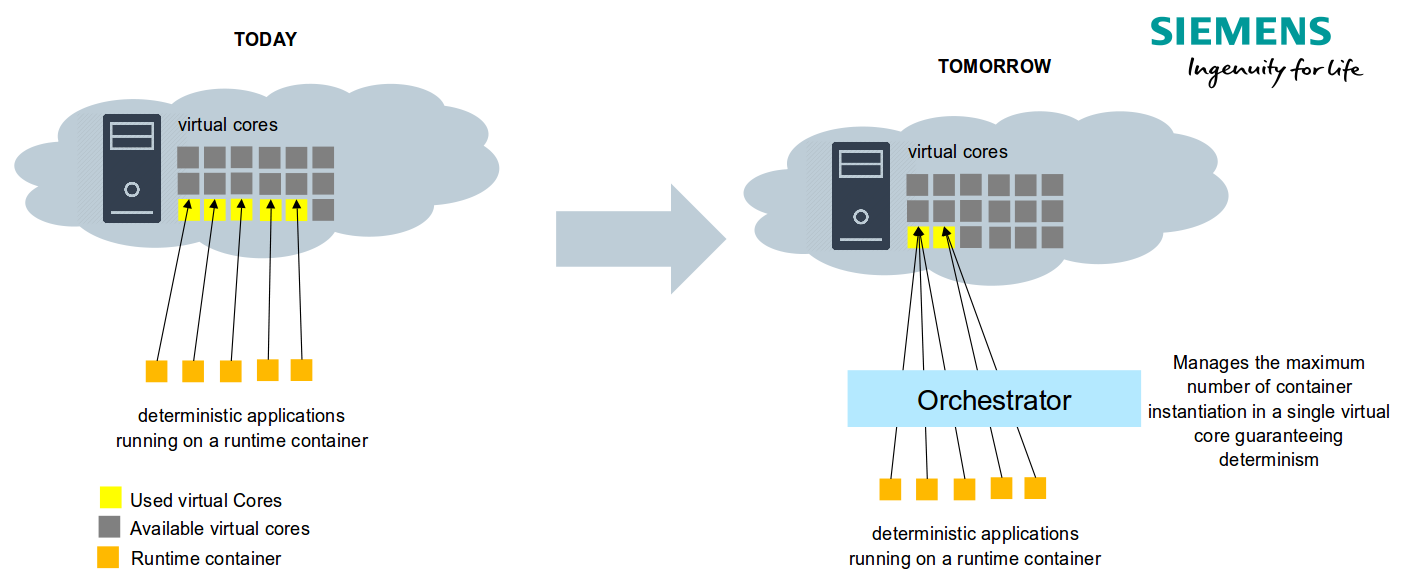
\includegraphics[width=0.8\textwidth]{plan}
	\caption{Planned resource re-allocation}
	\label{fig:plan}
\end{figure}

It is planned that this re-organization will save a major amount of resources, reducing the costs needed to operate the system while still being appropriately deterministic. 
To isolate the different applications from one-another, a containerized approach has been chosen beforehand. The main choices available are LXC/LXD, Docker and Balena.

LXC/LXD is the default Linux-based containerization engine. In its first release LXC was released as set of tools which are rather low level. The new extension LXD offers now a more intuitive approach, comparable to the more user-friendly Docker. LXC was rather difficult to use at first, probably one of the reasons why containerization did not take off until Docker came in. Docker is an open source project written in Go that is based on LXC technology. It has centralized container image storage, an open API and easy to use CLI interface\footnote{see \cite{docker01} for a full list of features}. Balena on the other hand is a stripped down version of Docker, allowing to minimize the resource requirements. It is an open source project hosted by resin.io. It uses the Docker infrastructure and has therefore a lot of its advantages while diminishing the load for the system. Balena kept most of the same configurations and parameters allowing a switch to Docker and its more advanced features at any time. For this reason, at the initial meeting of the 25-26/08/18 (see meetings in Section \ref{sec:meeting}), Balena has been chosen as the containerization engine. 

\section{System Tests and variants}

{\small\textsc{Identification of application candidates, 25-30/07/18} \bigskip}

Before selecting a specific setup, different variants of systems are tested for their real-time capabilities, maintainability and ease of setup.
Through some keyword browsing a list of potential systems has been identified.
Candidates for this session are:

\begin{itemize}
	\item \textbf{resinOS} operating system by \textit{resin.io}, designed to run containers on different architectures and hardware devices. It has Balena pre-installed and features a cloud based interface to manage the different hosts and running containers.
	\item \textbf{Ubuntu Core} an operating system for IoT devices implemented using the new snap image approach. Snap based as well as Balena based approaches are investigated on this hardware optimized image
	\item \textbf{Xenomai 3} is co-core extension for Linux based operating systems, which allows hard-real-time scheduling. Together with an interrupt pipeline patch it is suggested to be the most performing of the real-time approaches.
	\item \textbf{PREEMPT\_RT} a kernel patch for Linux-based systems which increments the achievable preemption level of the kernel. This allows for soft- and firm-real-time based performance, reaching hard-real-time on a properly tuned system
\end{itemize}

CoreOS has been excluded from the candidate list as it comes with a LXC/LXD image and is stripped down to the bare minimum (LXC/LXD has been excluded beforehand).
The systems are setup in separate virtual machines and are verified for real-time scheduling properties. The performed test  installations will be used to verify the run-time behavior of containerized applications of different kind, including synthetic applications.

\subsection{resinOS by Resin.io}

{\small\textsc{Test-run resinOS, 25/07/18} \bigskip}

\textit{resinOS} is an Project-Yocto based operating system designed by ``resin.io'' to run containerized applications on small systems. The design also includes a cloud based monitoring infrastructure where the different configured devices connect to. The default containers supplied by resinOS are based on the lightweight general purpose Alpine Linux.

\subsubsection{Local Virtual Machine}

The resinOS operating system was primarily made to run on low resource systems, embedded devices or alike, and does thus not have a specific image for desktop/laptop or server. To run the OS in a virtual machine we download the Intel based 64 bit image for the Intel NCU industrial unit from the resinOS website \cite{resin01}.

The image does not contain any additional configuration concerning network setup or ssh keys and thus by default is not possible  to connect to the device.
To configure the image we need the CLI tool. Before installing the tool, make sure that following packages are present and configured:

\begin{itemize}
	
	\item \textbf{node.js 6.x} you can install the latest version via snap using \textit{snap install node --classic --channel=x} where x can be substituted with the desired version, 8 or 10. You can also use a standard package installation. Instructions can be found at \cite{node01}
	\item \textbf{npm} the node package manager is part of the node distribution. If not yet installed, install it with \textit{apt-get install npm}
	\item \textbf{rsync} versatile remote file copying tool, installable, if not already present, via \textit{apt-get install rsync}
	\item \textbf{ssh} the secure shell client is usually pre-installed on all debian based systems. If that is not the case, install it via \textit{apt-get install openssh-client}
	
\end{itemize}

Once verified that all needed software is installed, the CLI tool for resin can be added using the node package manager. Please note the need of proper privileges (sudo).

\begin{verbatim}
	npm install --global --production --unsafe-perm resin-cli
\end{verbatim}

The CLI will now allow us to configure the image as needed. For a guided configuration, and assuming the downloaded image is in \textit{~/Downloads}, type the following 

Configure the image as needed
\begin{verbatim}
	sudo resin local configure ~/Downloads/resin.img
\end{verbatim}

Manual configuration instructions and further details and documentation can be found at \cite{resin02}.
 
Before the image can be deployed to a virtual machine, it has to be converted to a virtual disk image. 
Use the Virtual-Box CLI tool to execute the conversion. Once switched to the folder where the image has been downloaded, type
\begin{verbatim}
	VBoxManage convertdd resin.img resin.vdi
\end{verbatim}

Next, create new virtual machine in Virtual-Box based on ``Other Linux 64bit''. Minimum requirements are OK. Create a virtual Disk of Size of at least 4GB as main disk. 
When created, open the settings dialog for the virtual machine. In general settings, set the parameters as in Figure \ref{fig:resingen}. Now add the boot image for resinOS in the storage menu, Figure \ref{fig:resindisk}.

\begin{figure}[t]
	\centering
	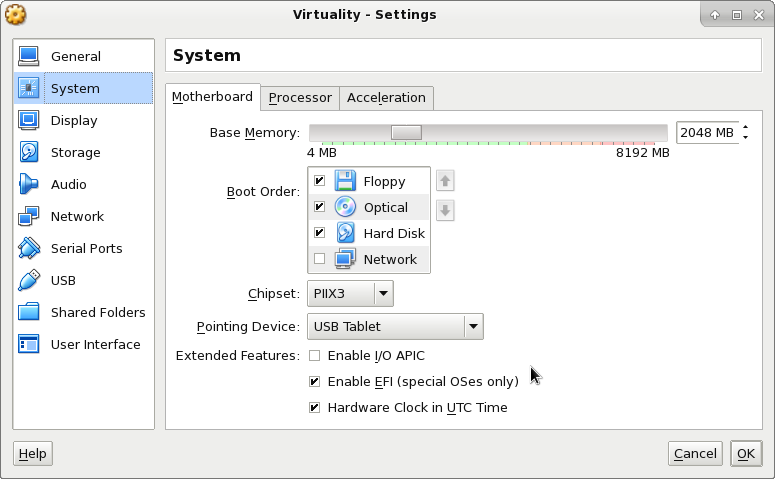
\includegraphics[width=0.8\textwidth]{resin-vbox}
	\caption{Virtualbox general settings for resinOS}
	\label{fig:resingen}
\end{figure}

\begin{figure}[t]
	\centering
	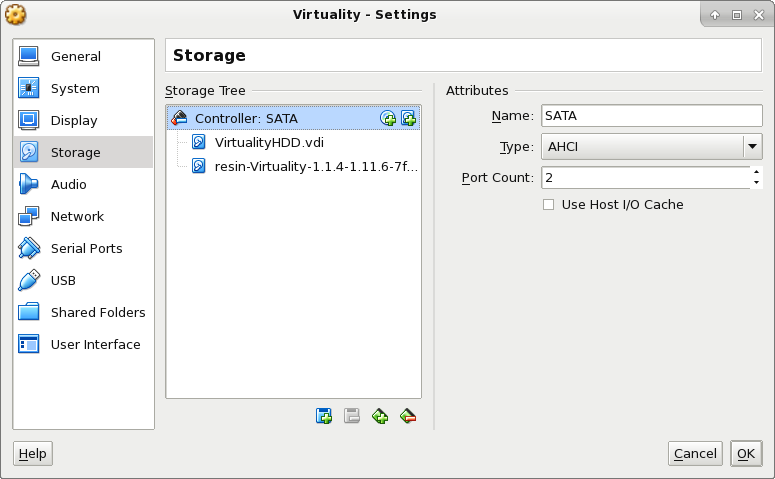
\includegraphics[width=0.8\textwidth]{resin-vbox2}
	\caption{Disk settings for resinOS}
	\label{fig:resindisk}
\end{figure}

To properly connect and download eventual containers we have to configure some port forwards. In the ``Network'' menu, select advanced, then Port forward. Configure now the forward of host port 8022 to client port 22 and host 2375 to client 2375, both for the client IP 10.0.2.15 (usually). The host IP can be left blank.

If the virtual machine is now started, the downloaded boot image creates a new instance of resinOS on the previously created virtual drive. The new disk is populated with the settings specified in the configuration step. Once done, the system shuts down automatically and the resin boot image can be removed from the machine settings. At next boot, the new virtual disk is used as boot image.

\subsubsection{Run a Balena container in resinOS}

As already discussed before, \textit{resinOS} is shipped with Balena pre-installed and the system is now ready to run any desired container. 
An example application responding to a simple web request can be set-up and tested with the following guide.

Clone the repository to a local directory with
\begin{verbatim}
	git clone https://github.com/resin-io-playground/resinos-sample
\end{verbatim}

Now enter the repository and edit ``Dockerfile''. Replace the text after FROM with \textit{resin/intel-nuc-alpine-node:slim}. Now compile and upload the container to the virtual host with

\begin{verbatim}
	sudo resin local push localhost --source .
\end{verbatim}

Setup a route from the virtual machine to the local host, line before, from port 80 to port 8080. Browsing to \texttt{localhost:8080} should now display a test page.

\subsubsection{Evaluation}

The resinOS core ships with no packager manager and is missing building tools. This image can therefore be patched only manually and with greater effort. This also means that it increases the maintenance effort and makes thus a resinOS based approach unpractical. In addition, the image has been tuned for small devices' operation. An operation on a server infrastructure would therefore not use the maximum capabilities of the hardware, constraining the system in its performance.

\subsection{Ubuntu Core}
{\small\textsc{Test-run Ubuntu core, 25/07/18} \bigskip}

Ubuntu Core is a project to bring small applications to embedded devices based on standard Ubuntu technology. The developed software is shipped in a snap and then run sand-boxed in a container-like environment while keeping the transparency of a traditional application. 

Snaps are standard feature of Ubuntu based distributions since 2 years now. It combines the advantages of a package manager and a virtualized container. Even though the snap itself runs on isolated resources provided through proper \texttt{cgroup} configuration, it maintains the accessibility and transparency a locally installed software would have. 
The running applications are practically sand-boxed, having separated partitions for binaries, application specific settings, and the actual file system of the host OS. The host and the binary partitions are read-only, protecting the hosting system from eventual malicious software. 
In addition, the binaries are digitally signed and thus tampering with the executable is avoided. This gives the whole system the flexibility of continuous updates of an application while being independent of the host system and flavor, and without interacting with the file system of the host.
A variety of Linux flavors support snaps. In addition, snap-stores can be privately hosted, making this solution very interesting. More details can be found at \cite{snap01}

In this test, a setup is described and feasibility of the candidate is verified.

\subsubsection{Local Virtual machine}

Like in the previous example, the image is downloaded and ready to be used. Visit \cite{ubuntu01} for an additional step-by-step guide.
First, we get and unpack the latest KVM core image (replace version numbers where appropriate):

\begin{verbatim}
	wget http://cdimage.ubuntu.com/ubuntu-core/16/stable/current/ubuntu-core-16-amd64.img.xz
	unxz ubuntu-core-16-amd64.img.xz
\end{verbatim}

Before it can be used, the image has to be converted from a raw image to a virtual drive. We convert the image again with the VirtualBox CLI tool.

\begin{verbatim}
	VBoxManage convertdd ubuntu-core-16-amd64.img ubuntu-core-16-amd64.vdi
\end{verbatim}

Now we create a new virtual machine based on ``Ubuntu 64bit'' and add the existing disk. The setup of the virtual machine is guided and therefore no additional description is given here. Standard settings are good enough. Once done, the system is ready to run.

In order to be able to connect to the new virtual machine we need a Ubuntu one account. In the account we then specify the ssh key we are going to use to connect to the core device. The booted device will ask the email of the Ubuntu one account and subsequently download the ssh key. 
Finally, to connect via ssh we have to configure some forwards. In the settings, select ``Network'', advanced, then Port forward.
Configure now the forward of port 8022 to 22 for client host 10.0.2.15 (usually), the same way as described for resinOS.

For a description on how to create a ssh key, visit \cite{atlassian01}

\subsubsection{Evaluation}

Unfortunately, as for resinOS, also Ubuntu core is stripped to minimum and ships with no packager manager and building tools. Therefore, the same conclusions as before apply.

Unfortunately, even though the snap feature is native to Ubuntu and a patched kernel could add the needed real-time properties, the binding with the hosts name and file-space hinders the use of application duplicates. This approach is thus archived for the moment.

%If all other attempts are not successful enough, a conversion of the apps to snaps and proper configuration might be considered.

\subsection{Ubuntu Server 16.04.4 with Xenomai}

{\small\textsc{Testrun Xenomai, 26/07/18} \bigskip}

Xenomai is an OS extension which can be used to support POSIX real-time calls in a standard Linux kernel. 
Xenomai integrates it with Cobalt, a small real-time infrastructure which schedules time-critical activities independently of the main kernel logic. 
The interaction with an interrupt dispatcher (I-pipe) allows to increase response time and performance and thus enables also for hard-real-time execution. 
Through further extension with interface skins, also non POSIX compliant real-time software can be configured to run on a Xenomai patched system.

The main expressed concerns of this approach are setup complexity and maintainability.

\subsubsection{Local Virtual machine}
\label{sec:xenoinst}

The base-OS should be lightweight but still fully featured. Thus, an Ubuntu server flavor with minimal installation has been chosen. 
Download the image from the Ubuntu website \cite{ubuntu02}. The latest patches available for Xenomai/I-Pipe are based on Kernel 4.9.x and 4.14.x. Ubuntu 16.04 is the closest version with 4.4.x as the next LTS, namely Ubuntu 18.04, is shipped with Kernel 4.15.x. 
Thus, we select Ubuntu Server 16.04.4 as the candidate for a kernel upgrade and patch.

\begin{verbatim}
	# download image
	wget http://releases.ubuntu.com/16.04.4/ubuntu-16.04.4-desktop-amd64.iso
	# verify image hash
	curl -sfL http://releases.ubuntu.com/16.04.4/SHA256SUMS
	|	sha256sum -c 2>&1 | grep OK
\end{verbatim}

Next, we create a new Ubuntu 64bit based virtual machine with a disk size of at least 20GB. 
Even though Ubuntu takes just a few GB, we need at least 10GB extra space for the libraries, source code and compiling process of kernel image and header. 
The memory size for the virtual machine can be arbitrary chosen between 384 MB and $\inf$. When setting the number of assigned CPUs, consider that the more, the faster is the compiling of the new kernel (upper limit, of course, are the physical no of threads). 
If you increase the number of CPUs, increase also the amount of RAM.
Before starting the machine, we add the Ubuntu server disk image to the CD drive of the new machine.

Now follow the guide of the installer. If asked, add only ssh server to the pre-selected packages and continue with software deployment. 
Once the installation is done, don't forget to upgrade the system to the newest packages and restart before proceeding with the kernel build.
Execute the following in the freshly booted system:

\begin{verbatim}
	apt-get update && apt-get dist-upgrade -y
\end{verbatim}

The patching steps have all be resumed in an installer script by Pasquale Antonante. Unfortunately some steps are outdated and some configurations have changed.
The script has therefore been updated and placed in the appropriate directory of this repository \cite{gitrepo}. 
The install script provides automatic downloads of the two patches, Xenomai/Cobalt and I-Pipe, the kernel, performs the patch and installs new kernel and the Balena environment.

\subsubsection{Evaluation}

Because of the way interrupt handling is implemented, using out-of-band interrupt handlers and thus immediate IRQ reception, Xenomai is an ideal candidate for hard-real-time applications. 
The patching is bound to kernel versions, thus the progress depends on the patch development of I-Pipe. 
The scheduling of the real-time tasks is performed in the co-kernel and is thus easier to modify and change, a promising approach.
Currently the kernel patch development line (incomplete) is stuck at version 4.14.4 (the latest kernel shipped with Ubuntu 16.04 LTS is 4.15.0-29, the latest stable 4.17.11). 
This could be a sign of an abandoned project. Before continuing with this implementation line, a proper investigation of the project status and agenda must be performed.

\subsection{Ubuntu Server 16.04.4 with patch RT}

{\small\textsc{Testrun Preempt-RT, 27/07/18} \bigskip}

PREEMPT\_RT is a real-time kernel project maintained by the Linux foundation. 
The main aim of the PREEMPT\_RT patch is to minimize the amount of kernel code that is non-preemptible. Therefore, several substitutions and new mechanisms are implemented.
In the last years there were some major improvements in the PREEMPT-RT performance. A paper of Fayyad-Kazan \textit{et al.} shows improvement on kernel versions v2.6.33 versus v3.6.6 of a total of 35\% \cite{Fayyad-Kazanetal2014}. In order to keep performances and results comparable, preferably the same Ubuntu image as for Xenomai will be used for patching.

\subsubsection{Local Virtual machine}

The same conditions as in the previous example apply. Download the image from the Ubuntu website \cite{ubuntu02}, if not already done. See section \ref{sec:xenoinst}.

The patching steps have all be resumed in a newly created installer script similar to the previous case with Xenomai. The install script provides downloads of the patch and the kernel, performs and installs the patch and installs the Balena environment.

For further guides on how to compile and install a kernel, visit \cite{misc01}.

\subsubsection{Evaluation}

The Preempt-RT requires a dedicated patch, recompiling and tuning of the kernel to support hard-real-time properties. The additional slicing preformed to the kernel tasks allows faster preemption and a better control of the CPU scheduling.
Compared to the previous example, the handling of interrupt flow can not be controlled to the same extend reaching thus a lower real-time guarantee.
In particular, drivers must be tuned for real-time operation in order to reach low process firing jitter.
Anyway, lately the project has made remarkable progress.
Its mainline development is following kernel distribution at a fast pace, indicating that the project is strongly followed and has a valuable community backup. This makes the solution a major candidate for further investigation.
To exploit its full potential, newer kernel patching as a future step is taken into consideration.

\section{Tests of system}

{\small\textsc{Test-run and comparison of systems, 30/07/18} \bigskip}

Some small cyclic execution tests are performed to verify default availability of real-time scheduling and the timing behavior of the scheduler. Some tools will be downloaded and installed to test for latencies, responsiveness and reaction under CPU stress. 

\subsection{rt-tests}

The rt-tests suite includes a list of small tool binaries which may be used to test properties of real-time systems. The most known are \textit{cyclictest} and \textit{hackbench}.
The former is used to create a number of real-time tasks executing periodically which then report their starting latencies. 
The latter has specific features to backtrack also single latencies (\texttt{--breaktrace}), allowing to debug the latency trace of the preemption kernel. 
It is a feature that requires a specific kernel configuration and might thus be used in a second moment, i.e. when configuring the container host OS. 
To install the software we may use one of the two approaches:

1) We use Xenomai 2.6.x (which is not our case), then there is a ready to go tool package available

\begin{verbatim}
	apt-get install xenomai-system-tools
\end{verbatim}

2) We use another version or real-time approach and compile the binaries from the source code.
For this approach we need first some additional packages. Get them with: (\textbf{Note:} for Xenomai 3.x check new findings in Section \ref{sec:isol} before continuing)

\begin{verbatim}
	sudo apt-get install build-essential libnuma-dev
\end{verbatim}

Now proceed with the installation. Download the git repository and compile the source.

\begin{verbatim}
	git clone git://git.kernel.org/pub/scm/utils/rt-tests/rt-tests.git
	cd rt-tests
	git checkout stable/v1.0
	make all
	make install
\end{verbatim}

The last step is optional. The binaries can now be run (within the directory) to perform the different tests. An example of a test recommended by Kernel.org is: 

\begin{verbatim}
	cyclictest -t 50 -n -d 86400 -l 100000 -a -p 99
\end{verbatim}

The code in the example creates fifty tasks with priority 99 (maximum) an interval of 1000 $\mu s$ and a task period distance of 86400 $\mu s$ and using a clock-based nanosecond timer.
An interesting feature is the \texttt{-h} flag, which plots a histogram and the number of overshoots. The feature will be used in a second moment.

As an example, we compared the results between virtual machines of the different kinds we have set up by now. There is an improvement between normal and patched images, but the actual values are for now far from ideal. 
At the moment, as the host is not hard-real-time capable, the delays also depend on the scheduling of the host which runs the virtual machine. Thus, even though an eventual cloud host is not hard-real-time capable, an additional series of tests with such a host could give some more comparing and reference data.

\subsection{stress}

In order to verify behavior also under stress we use the tool \textit{stress}. The tool starts some random computation in order to put load on the virtual machine. 
The installation can be performed by downloading and compiling the source code. Further information can be found at \cite{stress01}.

\begin{verbatim}
	#download and extract
	curl -sfL http://people.seas.harvard.edu/~apw/stress/stress-1.0.4.tar.gz | tar xvz
	# compile and install
	cd stress-1.0.4
	./configure
	sudo make install
\end{verbatim}

An example execution starting three threads of each function of stress can be performed via the command:

\begin{verbatim}
	stress -d 3 --hdd-bytes 20M -c 3 -i 3 -m 3 --vm-bytes 15M
\end{verbatim}

\subsection{Other testing tools}

A list of other tools that might be helpful:

\begin{itemize}
	\item \textbf{htop} a colored memory view to analyse memory use of single processes
	\item \textbf{iftop} interface monitor to view actual network traffic
	\item \textbf{iotop} generic I/O monitor
	\item \textbf{nmon} a universal monitoring tool
\end{itemize}

\section{Additional fixes}
{\small\textsc{Configuration test, 31/07/18} \bigskip}

Balena, even though installed via the official script, appears not properly configured. It does not run at startup and there is no typical dedicated group in order to ease and limit access to the engine.
Therefore, groups and systemd configuration files to manage these must be added manually. Use the Docker reference manual to provide for this. The manual can be found at \cite{docker02}. The Balena daemon is started via the command \textit{balenad}.

\begin{figure}[t]
	\centering
	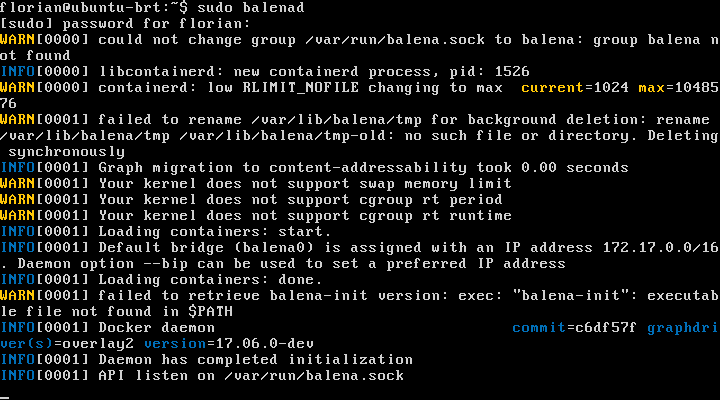
\includegraphics[width=0.8\textwidth]{balena-err}
	\caption{Error messages displayed by Balena at first run}
	\label{fig:balenad}
\end{figure}

It is also unclear why the official installation script misses the \texttt{balena-init} file, see \ref{fig:balenad}. 
Comparing the installation to the standard resinOS shipping we can see that the latter has the mentioned file.  The two Balena engines have the same version number, but interestingly the main binary of the tool is different. 
It is unclear what this might mean. The init binary is intended to initialize a newly created container in order to remove all the orphaned resources and prepare it for a clean run. 

If we refer to documentation it just seems a forgotten installation step.
According to the Docker reference manual, \cite{docker03}, the init binary is obtained via \texttt{tini}, thus can be safely pulled from there. The git repository can be found at \cite{tini01}.

Figure \ref{fig:balenad} shows also a number of further warnings. In particular, we can identify two groups of warnings:

\begin{itemize}
	\item \textit{WARN[0001] Your kernel does not support swap memory limit}

	\item \textit{WARN[0001] Your kernel does not support cgroup rt period} and \textit{WARN[0001] Your kernel does not support cgroup rt runtime} 
\end{itemize}

The former is due to the fact that memory swap support has not been enabled at kernel built time. 
The configuration setting to be enabled is \texttt{\#CONFIG\_MEMCG\_SWAP\_ENABLED}. As a temporary fix we can enable the settings at boot-time. 
To do this we edit \texttt{/etc/default/grub} and set 
\texttt{GRUB\_CMDLINE\_LINUX\_DEFAULT} to \texttt{"cgroup\_enable=memory swapaccount=1"}

The latter of the two warning groups is also due to a configuration setting of the kernel. They concern the real-time run-time control of single cgroups. This is a feature which is needed/used in containers when we want to control a containers' maximum CPU execution slice, see \cite{docker04}. 
In fact, if we try to set some real-time settings on our running Balena instance we get the following error message: \textit{balena: Error response from daemon: Your kernel does not support cgroup cpu real-time runtime.}.
The required setting can be enabled at kernel compilation time via the \texttt{CONFIG\_RT\_CGROUP} flag. 
%
Unfortunately the flag can not be enabled for the PREEMPT\_RT version of the virtual machine. Due to some temporary compatibility constraints, the simultaneous operation of the \texttt{CONFIG\_PREEMPT\_FULL} flag, necessary for the ability of full kernel preemption, and the CGroup flag has been disabled. Details can be found at \cite{lfnd01}.

Finally, I found a script that could do the verification for you. If you would like to test your system for parameter and capability compliance, the Docker community has developed a configuration testing script. The test can be run via these inputs:

\begin{verbatim}
	wget https://raw.githubusercontent.com/dotcloud/docker/master/contrib/check-config.sh
	chmod +x check-config.sh
	./check-config.sh
\end{verbatim}

The run of the script confirms that the Xenomai version of the image, after all reconfiguration and recompilation, has the correct settings to operate the container engine with real-time features.

\section{Virtualization sustainability tests}
\label{sec:virtsust}
{\small\textsc{Test-run Containers \& CPU pinning, 01/08 - 03/08/18} \bigskip}

In this section we verify the real-time latencies in different settings and how the applications behave inside a container. In order to do this, a variety of system configurations are performed and capabilities verified. 
The list of all capabilities can be viewed on every Linux based system by typing \texttt{man 7 capabilities} into a shell. 
This tests should give an insight how a real-time container and/or application will behave when put into a virtualized environment like the Amazon AWS cloud. Amazon offers different setups, from shared or dedicated virtualized hosts to bare metal applications. 
The results will show how the set-up and configuration of a cloud and its  hypervisor (here the Host) could influence latencies and responsiveness of a real-time application running in a virtualized environment. 
According to Siemens, the target application will have a period $T$ of about $100 ms$, where computing time is expected to be in the range of $\frac{1}{10}^{th}$. This means, to achieve hard-real-time operation and not miss any deadline, the application latency should never exceed $\frac{9}{10}^{th}$ of the period, i.e. $90 ms$.

During some additional research on Balena and its relation to Docker, the source code of Balena actually revealed that Balena exposes the same API. Thus, the use and parameters for compose, namely \texttt{docker-compose}, is available to run also on a Balena based system.
\texttt{docker-compose} is a tool written in python which allows to configure and connect multiple containers remotely using a single Json file, a welcome feature for our project.
Anyway, by the source code of Balena we can tell that not all the tags are supported. This is particularly valid for the `Deploy' section. 

More detail on the different activities performed in this section and on why those are performed, can be found at \cite{lrt01}.

\subsection{Preparing steps}

In preparation for the upcoming tests we need to install \texttt{docker-compose}.
The instructions can be found in the reference of Docker, see \cite{docker05}. 
On Debian systems this can be done simply via 

\begin{verbatim}
	apt-get install docker-compose
\end{verbatim}

During these tests, the virtual machine is set to 3 CPUs, and the CPU affinity of the task on the host is set to 7 (CPU 0,1,2). This will allow to avoid task switching and further separate RT tasks (CPU 0-1) from nRT tasks (CPU 2) inside the virtual machine
In the settings of the virtual machine we set the CPUs to three, and we start the virtual machine.  

\subsection{CPU isolation and partitioning tests}

Let us try to start with some first measurements. We will run the tool \texttt{cyclictest} in different combinations, with and without stress on the CPU. 
During the test, we will use two versions, one with system load and one without. The \texttt{-q} flag on the \texttt{cyclictest} program is mandatory because if on-line, it continues to overwrite the values which could result in shifted, bigger looking results. 
The goal of this test is to find a configuration that permits a very low average latency and thus relatively the best performance in a vitualized environment.

\begin{verbatim}
	#Test without load
	cyclictest -n -a -m -q -p 99 -l 100000
	#Test with system load
	stress -d 3 --hdd-bytes 20M -c 3 -i 3 -m 3 --vm-bytes 15M &
	 cyclictest -n -a -m -q -p 99 -l 100000;
\end{verbatim}

The measurement result are then printed with the following schema
\bigskip

\noindent \small \texttt{T: 0 (<pid>) P:<p> I: <i> C: <c> Min: <n> Act: <a> Avg: <v> Max: <x>}
\bigskip

Where:
\begin{where}
	\item[pid =] threads PID,
	\item[p =] threads real-time priority,
	\item[i =] execution interval in $\mu s$,
	\item[c =] cycle count of execution
	\item[n =] min run delay in $\mu s$,
	\item[a =] actual run delay in $\mu s$,
	\item[v =] average run delay in $\mu s$,
	\item[x =] max run delay in $\mu s$.
\end{where} 

Tests will be repeated to confirm values also in different situations.

\subsubsection{First tests with host}

First of all, let us get some base measurements. The testing host is a dual core, 4 thread, sixth generation i7 Skylake (U) system with 16GB of RAM. The guest has been set-up to three cores
and started without any further change. 
Ultra-books and laptops often disable Hyper-threading to save energy when operating on battery (a power management setting). Thus, in order to have all threads running, plug-in the power chord before continuing.
In addition, in many cases the \textit{cpu-governor} controls the bus frequency even if plugged in. Thus, we change the governor settings running the following as root. 

\begin{verbatim}
	cpupower frequency-set -g performance
\end{verbatim}

Now the clock frequency should be locked between upper limit and turbo frequency (where available). Frequencies can be verified with \texttt{lscpu}. 

The cores are all enabled and the system is ready to perform.
We begin thus with the first two tests:

\bigskip

\noindent No load :

\noindent \small \#1 \texttt{T: 0 ( 1489) P:99 I:1000 C: 109551 Min: 0 Act: 4894 Avg: 1370 Max:  491481}\\
\noindent \small \#2 \texttt{T: 0 ( 1687) P:99 I:1000 C: 100000 Min: 0 Act:  186 Avg: 1877 Max:  818579}\\
\noindent \small \#3 \texttt{T: 0 ( 1689) P:99 I:1000 C: 100000 Min: 0 Act:  604 Avg: 1664 Max:  8927944}\\

\noindent Load:

\noindent \small \#1 \texttt{T: 0 ( 1731) P:99 I:1000 C: 100000 Min: 1 Act:   40 Avg:  311 Max:   11892}\\
\noindent \small \#2 \texttt{T: 0 ( 1748) P:99 I:1000 C: 100000 Min: 1 Act:   85 Avg:  292 Max:   27666}\\
\noindent \small \#3 \texttt{T: 0 ( 1765) P:99 I:1000 C: 100000 Min: 1 Act:  413 Avg:  290 Max:   11818}

\bigskip

The first values obtained without load show very high peak values and average delays bigger than the cycle times. On the other hand, the stressed run has a lower peak and delay times way lower than the cycle time. That is probably due to the continuous movement of tasks on different vCPUs in the first case. 
The low load allows the scheduler to fill up the CPU time with other threads and thus also to distribute them (load balance) between the vCPUs.
This movement of tasks causes registers to flush and L1-L2 caches will have to be refilled from L3. 
All this introduces latency which is visible in the average and peak values.
The guest under stress does not allow very much free CPU-time on the physical CPUs. Thus, the host treads are mostly run on the CPU thread not busy running the virtual machine. 
This prevents shifting of threads to other CPUs and the resulting added latency. As a consequence, even though the load on the system is higher, the overall performance is better. 

A conclusion that might be drawn from this is that, if the virtual guest in the could is run on shared physical CPUs, a similar scenario might occur. 
The standard Amazon AWS instance uses a Complete Fair Scheduler (CFS), the same type of scheduler used for standard Linux threads in our testing host \cite{xen01}.
Therefore, in such case, either the resources for the virtual machine are all allocated to a reasonable extent with real-time applications, or the system might require some added stress, like in this test, to force the host scheduler into a more predicable behavior. 

\subsubsection{Working with host CPU isolation}

CGroups is a standard Linux feature used for resource partitioning and CPU pinning (affinity selection). It is one of the techniques also used by Balena \& Co. to isolate the containers from the host. 
It is a technique that might be used in combination with previous systems in order to increase their real-time properties. The tool \textit{cpuset} allows to perform a lot of the manual steps needed in an easier manner. 
Thus, in order to give the virtual machine proper computing power, isolate it from the host processes, and to allow isolation of the real-time tasks from non real-time processes, we will now set up CPU isolation for the host CPU.
This change should bring the virtualization host closer to the actual AWS system. The hosts threads are usually not mixed with the clients threads, although in a best effort setting the physical CPU might be shared with another virtual instance.
In the latter case, the considerations taken in the previous section might become useful again.

A two core machine will usually have four vCPUs, meaning two cores and two threads per core which equals 4. Thus, we will assign vCPUs 0-2 to the virtual guest and CPU 3 for the host system.

First of all we need to install the \texttt{cpuset} utility on the host system. This can be done via:

\begin{verbatim}
	apt-get install cpuset
\end{verbatim}

Next we set-up the CPU-isolation. Open a process monitor, e.g. the system monitor, and get the PID of the running virtual host, the service and the pcd thread. Open a shell and change to root (or use sudo):

\begin{verbatim}
	cset shield -c 0-2 -k on --shield &&
	cset shield --shield --threads --pid <read-pid,read-pid>
\end{verbatim}

The virtual machine and all tasks depending on it are now moved to a separate control group named \texttt{user} which has exclusive access to the vCPUs 0 to 2. 
All tasks of the host, where possible, have been moved to vCPU 3 in the new group \texttt{system} (verify with \texttt{cset shield --shield -v} and \texttt{cset shield --unshield -v}). In Figure \ref{fig:test-cpu} the effect on the host of cpu-isolation is shown.

\begin{figure}[t]
	\centering
	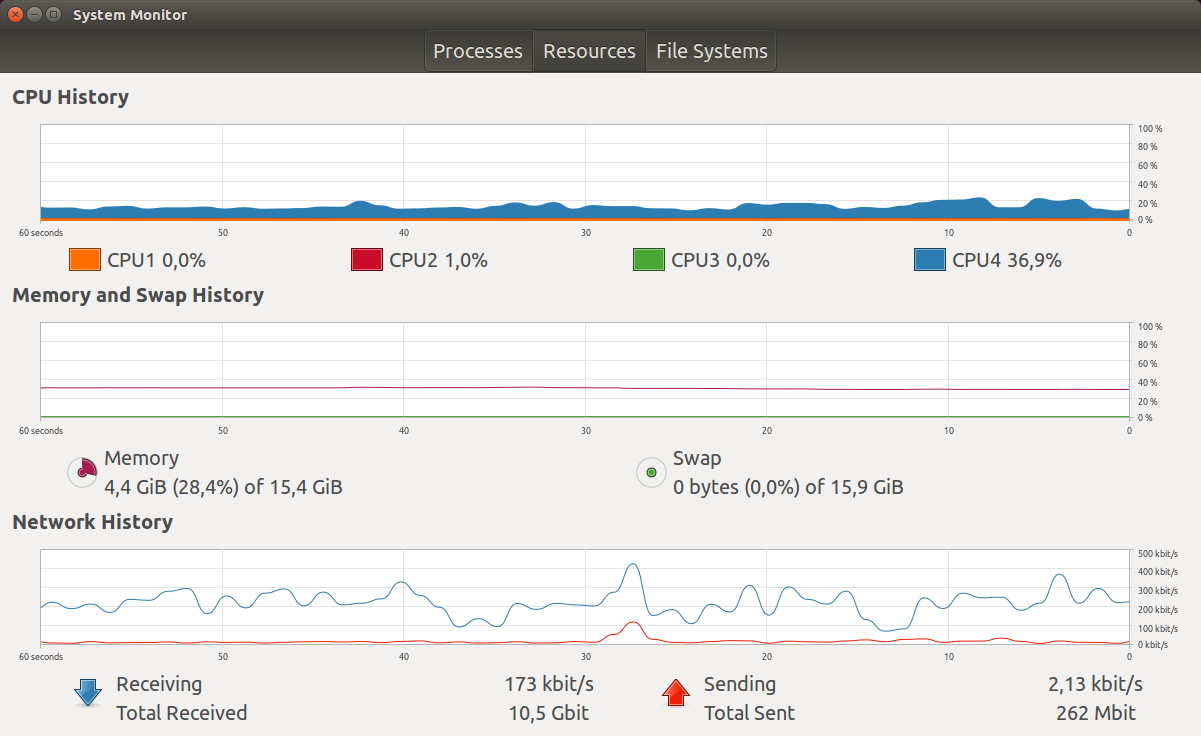
\includegraphics[width=0.8\textwidth]{test-cpu}
	\caption{System monitor showing the isolated virtual machine (idle) and the loaded host vCPU}
	\label{fig:test-cpu}
\end{figure}
\bigskip

%%%%% Cheklist tests
% shield installed onto all vbox processes?
% laptop powered and battery full?
% load balance ok?
% irq shifted? 
% life verifying of cpu load

\noindent Results with CPU isolation:

\noindent \small \#1 \texttt{T: 0 ( 1431) P:99 I:1000 C: 100000 Min: 0 Act:  263 Avg: 1319 Max:  761816}\\
\noindent \small \#2 \texttt{T: 0 ( 1615) P:99 I:1000 C: 100000 Min: 1 Act: 4387 Avg: 9382 Max: 1102853}\\
\noindent \small \#3 \texttt{T: 0 ( 1710) P:99 I:1000 C: 100000 Min: 1 Act:  156 Avg: 5043 Max:  976019}\\

%\noindent \small \#4 \texttt{T: 0 ( 1769) P:99 I:1000 C: 100000 Min: 0 Act:  139 Avg: 1075 Max:  822142}\\
%\noindent \small \#5 \texttt{T: 0 ( 1773) P:99 I:1000 C: 100000 Min: 0 Act:   78 Avg: 1660 Max:  963162}\\
%\noindent \small \#6 \texttt{T: 0 ( 1962) P:99 I:1000 C: 100000 Min: 1 Act:  116 Avg: 6758 Max:  769945}\\

With isolation, and still running a single real-time thread, the average delay is in some cases almost ten times the cycle time, causing the test duration to shift from planned 100 seconds to over 16 minutes. The values are very different and seem to vary based on the system load. 

One reason could be that, even though CPU affinity is set as parameter in the test, load balancing is still active. The host does not see the internal affinity settings of the virtualized guest. He only sees some threads to be executed.
Thus, the test-thread could be shifted in the host onto other vCPUs to keep the average workload balanced. This is the same case as before where the CFS tries to distribute running tasks equally among the available vCPUs.

Thus, in this second test, let us put again the virtual machine under load. If the previous theory is correct, an improvement on average and max values should be seen. The system's CPU load can be seen in Figure \ref{fig:test-cpuload}. It is as expected balanced on the three vCPUs dedicated to the virtual guest.

\noindent Results with added load: 

\noindent \small \#1 \texttt{T: 0 ( 1358) P:99 I:1000 C: 100000 Min: 0 Act:   49 Avg:  337 Max:   23395}\\
\noindent \small \#2 \texttt{T: 0 ( 2364) P:99 I:1000 C: 100000 Min: 2 Act:  201 Avg:  348 Max:   17171}\\
\noindent \small \#3 \texttt{T: 0 ( 2470) P:99 I:1000 C: 100000 Min: 1 Act:   38 Avg:  319 Max:   13496}
%\noindent \small \#4 \texttt{T: 0 ( 2577) P:99 I:1000 C: 100000 Min: 1 Act:   48 Avg:  345 Max:   16509}


\begin{figure}[t]
	\centering
	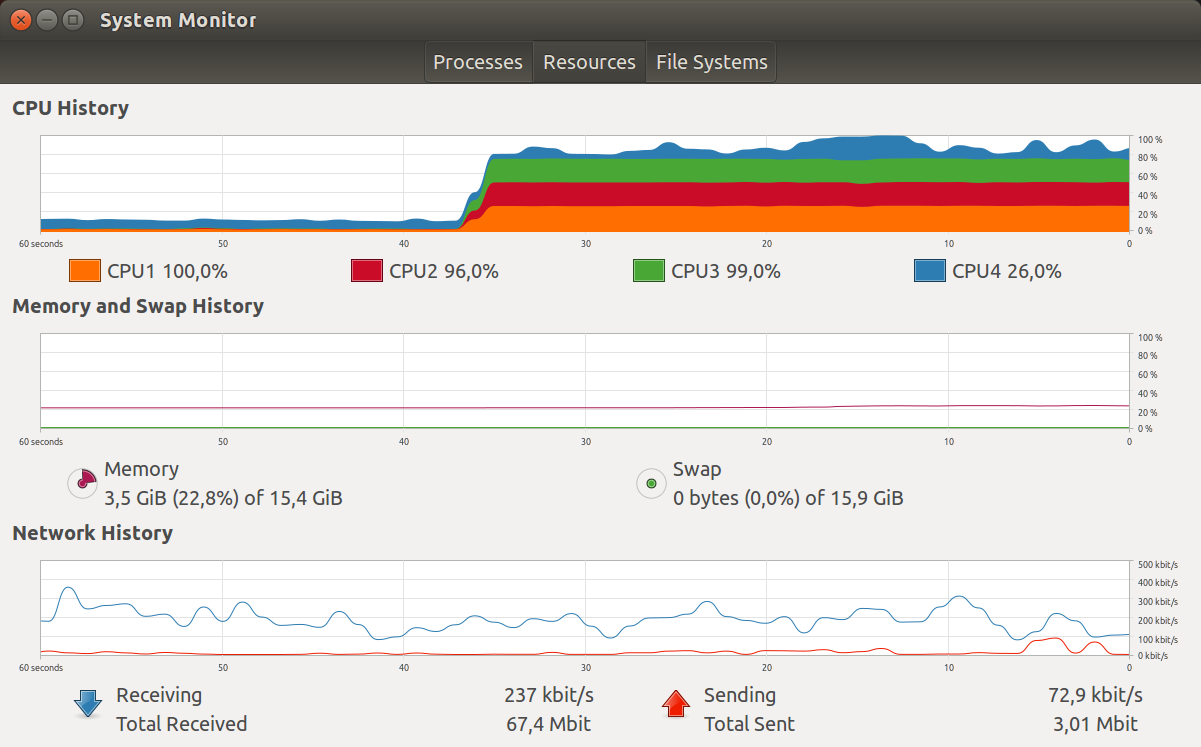
\includegraphics[width=0.8\textwidth]{test-cpuload}
	\caption{System monitor showing the same isolated virtual machine under load}
	\label{fig:test-cpuload}
\end{figure}

And, as expected, the average dropped way below one millisecond, confirming the previous theory.
Even though the threads of the virtual machine are confined on the tree vCPUs, the load balancer of on the host is still active. We test now what happens when we deactivate the load balancer on the host:

\begin{verbatim}
	#Removing load balancer total
	echo 0 > /sys/fs/cgroup/cpuset/cpuset.sched_load_balance
	#Removing load balancer shielded group
	echo 0 > /sys/fs/cgroup/cpuset/user/cpuset.sched_load_balance
	#keep load balancer system group
	echo 1 > /sys/fs/cgroup/cpuset/system/cpuset.sched_load_balance
\end{verbatim}
%\bigskip

\noindent Results without load balancer:

\noindent \small \#1 \texttt{T: 0 ( 1643) P:99 I:1000 C: 100000 Min: 1 Act:  345 Avg: 8740 Max:  968040}\\
\noindent \small \#2 \texttt{T: 0 ( 1805) P:99 I:1000 C: 100000 Min: 0 Act: 3004 Avg: 1705 Max:  792388}\\
\noindent \small \#3 \texttt{T: 0 ( 2096) P:99 I:1000 C: 100000 Min: 1 Act:   88 Avg: 6960 Max:  894669}\\

As we can see from the results, the values with and without load balancer did not change much.
At the moment it is unclear why this happens. For now, let us continue with the tests.

For now only the tasks, user or system, have been moved from their original CPU to vCPU 3. 
Interrupts on a multi-core system can be triggered on every active core and handled by the the specific routine. If our core serving the real-time thread has to serve the interrupt, the task has to wait.

In this next test we will move all possible interrupts to the last core. This should reduce the waiting time for the real-time tasks to be fired.
It is true that every system will always have some IRQ requests during run, but in this test we are trying ro reduce the effect of the hosts system interrupt to the virtualized tests.
On average, a slight improvement of the measurements should be visible.
Thus, to isolate further the virtual machine and move the IRQs only to vCPU 3 we can use the following command: 

\begin{verbatim}
	# move irq affinity to Cpu 3
	for file in /proc/irq/*; do   echo 8 > \$file/smp_affinity; done
	echo 8 > /proc/irq/default_smp_affinity
\end{verbatim}

\noindent The new test-results with moved IRQ affinity are then as follows:
 
\noindent \small \#1 \texttt{T: 0 ( 2151) P:99 I:1000 C: 100000 Min: 0 Act: 3481 Avg: 6496 Max:  892712}\\
\noindent \small \#2 \texttt{T: 0 ( 1625) P:99 I:1000 C: 100000 Min: 1 Act: 3294 Avg: 9001 Max:  933678}
\noindent \small \#3 \texttt{T: 0 ( 1966) P:99 I:1000 C: 100000 Min: 0 Act: 5380 Avg: 6599 Max:  928789}

Unexpectedly, the values continue to move in the range of multiples of the cycle-time. 
Other tests that now can be performed is to enforce the isolation even more. 
Until now we used the tool cpuset, which isolates vCPUs from their threads and gives exclusivity of access to certain cores only to threads that have been assigned to.
Now we will restart the cores (via the hotplug feature of the kernel) to force moving of tasks to the other cores. We will use the procedure described in \cite{lrt02}.

Following the description two things where noticed: 1) it is not possible to hotplug the cpu0 and 2) disabling CPU1 disables also CPU2 and CPU3.
While the former may be a convention in order to avoid disabling all CPUs, sometimes based on hardware \cite{lwn01}, the latter is an actual misbehavior. 
When checking interrupts via \texttt{cat /proc/interrupts} only vCPU1 is missing and assignment seems to work properly. Other CPUs hotplug function work properly. 
Thus, in order to be able to work with the instructions as of \cite{lwn01}, the reserved vCPUs will now be moved at the end of the range. 

The interrupt table gives us also some other information: almost all interrupts between 0 and 22 are allocated on vCPU2. This requires further investigation and is detailed in the next subsection.

\subsection{Problem isolation and repeating}
\label{sec:isol}

{\small\textsc{Unplanned review of results, 11/08 - 12/08/18} \bigskip}

Investigating the IRQ allocation in the Xenomai 3 version of the virtual machine, and comparing it to a standard machine, the allocation is completely different. This could explain the unexpected test results.

If we consider a single test thread that is run manually multiple times,on average only one out of three threads will run on the same vCPU.
As a test, if we try to pin the thread to the last CPU, the one which has the highest interrupt count, we get the following results: (Task pinning has been performed with \texttt{taskset -p 8 <pid-no>})

\bigskip

\noindent \small \texttt{T: 0 ( 1695) P:99 I:1000 C: 100000 Min:      0 Act:   73 Avg:  148 Max:    4773}

Interestingly, if we now deploy a thread on each CPU, including the last one, we get a very close result, but still worse than the thread on the last core.
This is reproduce-able also by changing the number of CPUs and the vCPUs assigned to the virtual machine. 
Only if we include the last one, or we pin on the last vCPU, we get an average performance under one millisecond. This phenomenon needs further investigation.

Working through the documentation again, it is described how code must be implemented and build with Xenomai libraries in mind. 
This means that for Xenomai to work properly, \textbf{all real-time code must be recompiled} with the proper libraries, \texttt{cyclictest} included.
Unfortunately this means, that all tests up-to now have been executed as soft-realtime linux applications and not in the Xenomai space.

The following must be included before compiling again the files in the rt-test repository: in line 5 of the \textit{Makefile} add

\begin{verbatim}
	XENO_CONFIG := /usr/xenomai/bin/xeno-config
	CFLAGS := $(shell $(XENO_CONFIG) --cobalt --cflags)
	LDFLAGS := $(shell $(XENO_CONFIG) --cobalt --ldflags)
	CC := $(shell $(XENO_CONFIG) --cc)
\end{verbatim}

If we run a test and verify the scheduled tasks with \texttt{cat /proc/xenomai/sched/threads}, we will see \texttt{cyclictest} listed as real-time application running in the cobalt scheduler.
Naturally, now all the tests have to be repeated with the recompiled file.

%what's this? Unknown origin
%\noindent \small \texttt{T: 0 ( 2615) P:99 I:1000 C: 100000 Min: 1 Act: 9296 Avg: 5138 Max:  7097944}

To confirm our conclusions, we use another tool called \texttt{latency}, part of the Xenomai library suite. First we perform a free-run test, then a test without load balancer on the host, and finally we move the IRQ affinity to the host-only CPU the same way described before. 
The results are displayed in table \ref{tab:latency}. The tool can be found in \texttt{/usr/xenomai/bin} and has to be run with the parameter \texttt{-p 1000} to set the period to 1ms (value of cyclictest).

\begin{table}[h]
	\caption{Running results using the  latency tool. All latency values are in $\mu s$}
	\begin{tabular}{l|r|r| r|r | r }
		Description &lat. min&lat. avg& lat. max&overrun& runtime\\
		\hline
% One core, no other settings 
%		1C 100$\mu s$ period&     -2.679&     10.937&  16748.829&   65932&    00:15:12/00:15:12\\
% One core, no other settings, 1000us
		1C&     -1.389&    190.744&  13008.966&   10782&    00:24:13/00:24:13\\
%two cores, 1000ms
		2C&     -4.194&  14028.789& 488841.139& 1100418&    00:20:22/00:20:22\\
%two cores, 1000ms iso
		2C iso&      0.715&  17216.756& 495533.945& 1759521&    00:31:30/00:31:30\\
% two cores, 1000ms iso, no load balancer
		2C iso nlb&      2.135&  19644.141& 239365.520&  901520&   00:16:14/00:16:14\\
% two cores, 1000ms, iso, noload, irq affinity
		2C iso nlb irq&      0.716&  21618.794& 492396.514& 2114650&  00:37:27/00:37:27\\
% two cores, 1000ms, no isolation, affinity vcpu 1
		2C aff&     -3.681&    212.699& 288657.832&    5882&   00:19:17/00:19:17\\
% two cores, 1000ms, iso, thread affinity to vcpu 1
		2C iso aff &     -1.627&    210.960&   7560.749&    1685&  00:14:25/00:14:25\\
% two cores, 1000ms, iso, noload, thread affinity to vcpu 1
		2C iso nlb aff &     -4.190&    219.501&   4843.218&    3899&    00:14:35/00:14:35\\
% two cores, 1000ms, iso, noload, irq affinity, thread affinity to vcpu 1
		2C iso nlb irq aff&      0.339&    174.257&   5064.610&    4476&   00:14:44/00:14:44\\

	\end{tabular}
	\label{tab:latency}
\end{table}

The description in Table \ref{tab:latency} indicates the number of vCPUS (C), if CPU shield was active (iso), no load balancer set (nlb), IRQ affinity re-configured (irq) or cpu execution affinity to the last vCPU was set (aff).

\subsubsection{Conclusions - isolation Host}
\label{sec:conciso}

We have seen in this first validation results that a VirtualBox task can be pinned to a certain CPU-set. Anyway, the results of the reaction times are varying with unclear reasons. 
One main reason could be that one of the vCPUs is not actually a separate core but only one of the two threads of the Hyper-threading instance of one physical core. 
Thus, it is possible that the increase in the max latency is due to the interrupt overload on the shared physical CPU, influencing thus directly the maximum performance and average latency of the real-time tasks.
In addition, as discussed in the VirtualBox Forum \url{https://forums.virtualbox.org/viewtopic.php?f=7&t=82721}, it is not possible to pin the single threads representing a vCPU to a physical CPU, even if shielded. It seems to be a situation isolated to the implementation of the standard VirtualBox hypervisor. 

The virtual machine in our example uses KVM paravirualizzation, the default setting for Linux in VirtualBox. 
KVM is a hypervisor which is actually supporting vCPU pinning. It might be thus possible to reconfigure the hypervisor by ovveriding VirtualBox settings to  finally allow the thread pinning and avoid the CFS scheduler of the hypervisor to shuffle the vCPU threads.
In any case, further tests with hypervisors such as native KVM supporting this feature is advised.

The results of the \texttt{latency} tool are very similar to the initial tests performed with \texttt{cyclictest}. With average values in the range of ten milliseconds and peaks up-to one second, the values are not yet good enough. 
Anyway, considering the test setup and constraints, and considering the application requirements, we can safely state that running applications with a 90ms admissible latency \textbf{is} possible. The load tests did show peak values under 30ms, a third of the maximum allowance. 
Thus, what is now to improve is the idle response time of the visualized instance. How much improvement is actually possible and what the various options will be matter of future work.

For the sake of completion, the tests will be continued using the same concepts of isolation also for the guest. It should help to predict the behavior of the cloud machine.

\subsubsection{Working with guest CPU isolation}

We now try to set-up the same isolation concept also for the virtual guest. The available cores are separated into real-time (RT) and non-real-time (nRT) groups. 
We will use one full physical core, 2 vCPUs, for RT and one virtualization thread, or one vCPU, for the nRT tasks such as standard operating system tasks. 
This way we can completely isolate the RT tasks on a separate core. The installation of the software \texttt{cpuset} is required like in the host case. We now shield and start the RT task in a isolated CPU group. 

\noindent Command : 

\begin{verbatim}
	# run shielding
	cset shield -c 0-1 -k on --shield
	# start test
	cyclictest -n -a -m -q -p 99 -l 100000
	# enable shield on test pid
	cset shield --shield --threads --pid <cycletest pid>
	# variant run shielded command
	cset shield --exec --threads -- cyclictest -n -a -m -q -p 99 -l 100000
\end{verbatim}

\noindent Results with CPU-isolation guest, no load balancer \& IRQ affinity set on host:

\noindent \#1 \small \texttt{T: 0 ( 1664) P:99 I:1000 C: 100000 Min: 0 Act: 3037 Avg: 1913 Max:  201188}\\
\noindent \#2 \small \texttt{T: 0 ( 2467) P:99 I:1000 C: 100000 Min:      0 Act: 4018 Avg: 1032 Max:   10262}\\
\noindent \#3 \small \texttt{T: 0 ( 1832) P:99 I:1000 C: 100000 Min:      0 Act: 3413 Avg:  222 Max:  201796}\\
\noindent \#4 \small \texttt{T: 0 ( 1835) P:99 I:1000 C: 100000 Min:      8 Act:  836 Avg:11725 Max:  718944}\\
\noindent \#5 \small \texttt{T: 0 ( 1869) P:99 I:1000 C: 100000 Min:      5 Act:   39 Avg:  222 Max:  199000}\\
\noindent \#6 \small \texttt{T: 0 ( 2243) P:99 I:1000 C: 100000 Min:      0 Act:   23 Avg:  158 Max:  200210}\\
\noindent \#7 \small \texttt{T: 0 ( 2246) P:99 I:1000 C: 100000 Min:      8 Act:   32 Avg:12487 Max:  674647}\\
\noindent \#8 \small \texttt{T: 0 ( 2257) P:99 I:1000 C: 100000 Min:      8 Act:10152 Avg:11605 Max:  765366}\\

In the results we can actually notice when the task is running on the last vCPU (chosen by the scheduler in round robin) or not. The tests with averages under one millisecond have actually been found to run again on the last vCPU. 

After we put load balance and IRQ affinity settings of the host back to normal, keeping CPU isolation we get the following results:

\bigskip

\noindent Results with CPU-isolation guest, load balancer and IRQ back in place for host:

\noindent \#1 \small \texttt{T: 0 ( 1912) P:99 I:1000 C: 100000 Min:      8 Act: 1898 Avg:14618 Max:  838961}\\
\noindent \#2 \small \texttt{T: 0 ( 1924) P:99 I:1000 C: 100000 Min:      8 Act: 9826 Avg:14524 Max:  847310}\\
\noindent \#3 \small \texttt{T: 0 ( 1934) P:99 I:1000 C: 100000 Min:      8 Act: 9569 Avg:14566 Max:  844467}

The test shows that isolation on the host actually influences the latency test in the guest.
Now, in addition we set the load balancer and irq affinity ion the guest to see if the performance improves. Remember to use value 4 this time for CPU affinity of the IRQs.
\bigskip

\noindent Results :

\noindent \#1 \small \texttt{T: 0 ( 1974) P:99 I:1000 C: 100000 Min:      8 Act: 9565 Avg:15748 Max:  858912}\\
\noindent \#2 \small \texttt{T: 0 ( 1979) P:99 I:1000 C: 100000 Min:      8 Act: 9638 Avg:13784 Max:  826807}\\
\noindent \#3 \small \texttt{T: 0 ( 2047) P:99 I:1000 C: 100000 Min:      5 Act:39152 Avg:13109 Max:  845584}\\

When changing load balanacer and IRQ affinity the values remain in the same range. It seems that the CPU isolation and configuration of the guest settings either has no impact or worsens the performance.
Thus, for the moment, the shielding and isolation of resources in the guest system will not be considered. 
Anyway, some final tests with a dedicated server should be performed to confirm this conclusion.

\subsection{Full dynamic ticks}

A thing not evaluated yet are full dynamic ticks (see \cite{lrt02}). To achieve full dynamic ticks on a CPU, there are some requirements on the application being run on this CPU. First of all, it must not run more than one thread on each CPU. The use of POSIX timers is also not allowed, directly or indirectly, which means that no kernel calls that require such timers, i.e. network access, and many others. Thus keeping the kernel calls at a minimum at the application itself increases the probability that a full dynamic tick system is achieved.
Second, the application must utilize the CPU partitioning, with e.g. \texttt{cset} done in previous section. After this, the shell command \texttt{taskset} can be used to bind the task to a specific CPU (task affinity) in the RT partition.

Anyway, by just by specifying ``more than one thread on each CPU'' we can exclude this approach upfront. We want to have more than one real-time application per CPU in order to save resources, thus, this configuration option is discarded.

\subsection{Tests Balena container}

Studying the Balena/Docker manual it was possible to identify the parameters to use in order to run the daemon with real-time capabilities. The parameter \texttt{--cpu-rt-runtime=<value>} enables the RT-sheduler for the daemon, set it to \texttt{-1} for no limit. In additon, for each RT-container \texttt{--cap-add=sys\_nice} must be set, while \texttt{--cpu-rt-runtime=<value>} and \texttt{--ulimit rtprio=<value>} can be used to limit run-time and priority for each container respectively.
More info at \cite{docker06}

By default, the daemon listens to the sock file only. To change this, and thus allow external access, we can specify the connecting interface where to listen to with \texttt{-H}. By default a virtual host has an IP address of \texttt{10.0.2.15}. To enable the debug mode, we can add the \texttt{-D} flag.

To start the daemon in real-time mode thus we use:

\begin{verbatim}
	balenad -H 0.0.0.0:2375 -H 10.0.2.15:2375 --cpu-rt-runtime=-1
\end{verbatim}

where 0.0.0.0:2375 stands for the default sock connection. Before we can connect from outside we have to add the usual port forward to the client IP 10.0.2.15 and port 2375 on both sides.

We can now run a test container with the real-time test program using the container setup in test-cont folder. The container has been setup creating a standard Dockerfile and a \texttt{docker-compose} file where the needed parameters are set. To upload the container do the machine, change into the container folder and type:

\begin{verbatim}
	DOCKER\_API\_VERSION=1.22 DOCKER\_HOST=tcp://localhost:2375 docker-compose up
\end{verbatim}

\textit{docker-compose} will now take care of downloading, building and running the image on the host.

\textit{docker-compose} foresees to specify a parent cgroup for each container. This means that we can group containers into resource blocks and then assign CPU, memory nodes and RT-runtime for each set of containers.
The parameters can either be changed via docker-compose file, the Docker command line or the standard cgroup virtual file system. An example of a run-time change for the main container root is the virtual file \texttt{/sys/fs/cgroup/cpu,cpuacct/docker/cpu.rt\_runtime\_us}.
The parameters of a child can not exceed the value of a parent. \textbf{Warning}, misconfiguration can severely destabilize a system. Generic information about real-time group scheduling can be found at \cite{kernel01}.

\section{Final considerations, Meeting decisions and updated remarks}

{\small\textsc{Study of further docs and sources, 06/08 - 07/08/18} \bigskip}

The test results, even if not as good as expected, showed that a real-time application with the given constraints might also be able to run with determinism in a virtualized host.
In addition, the study of the documentations of the involved technologies and tools brought additional information.
During my last investigation on \texttt{cgroups} and how they might be used in Docker/Balena, I bumped into a file that mentions, for the first time, an implementation of a Earliest Deadline First (EDF) based scheduler, \cite{kernel01}.
Following the description I found then in another text
(\cite{kernel02}) a discussion on a patch release going to be implemented on a mainline kernel version soon. Actually, there exist some recent papers which started to experiment with the EDF scheduler on a PREEMPT-RT patched system \cite{Buelnaetal2017}.
By further investigating on kernel source files on Kernel.org, and reading through sources, I found links to documentation \cite{wiki01} which stated that the completeness of the EDF is only recent.
\bigskip

``Since kernel 4.13, SCHED\_DEADLINE completed CBS with the Greedy Reclamation of Unused Bandwidth (GRUB) algorithm. The support has been developed by ReTiS Lab with the collaboration of Evidence Srl.''
\bigskip

Indeed, in the repository of the \texttt{chrt} standard scheduling tools \cite{schtools01} it can be seen that the version of tools starting from v2.28, version released with Ubuntu 16.04 is v2.27, permit input of  parameters for EDF scheduling.
This ,the late completeness of the scheduling option might be one of the reasons for the total lack of documentation.

In addition, the source code gave insight into another work in progress: the scheduling mode SCHED\_ISO. It is intended for fast interactive real-time tasks to be run for very short computation times. All in all, this suggests that the standard Linux scheduler  development is still ongoing.
It would therefore be interesting to exchange information with, if not take part, the main scheduling development team of the Linux kernel.

The study of the AWS system highlighted some recent changes. While the traditional systems are still based on XEN, which uses a CFS CPU scheduler \cite{xen01}, more recent virtual instance like the C5 use a new hypervisor based on KVM \cite{amazon01}.
This new hypervisor will allow direct assignment and control of hardware and resources.
This means, in short, that there is no need to use bare metal server instead: the new instances promise the same performance with greater flexibility and scalability.

In the last meeting it was finally decided to continue with Docker as a main virtualization platform and Kubernetes will be introduced as management tool for the virtualized machine and its containers.
One of the reasons is that, at the moment, the system of Figure \ref{fig:plan} is based on such technology and thus it would reduce the training cost of operators.
In sight of findings about the latest hypervisor development at Amazon AWS, in the meeting of the 07/08/18 we decided to operate on a C5 instance with at least 4 cores for the containers and, in addition, a generic instance for a Kubernetes monitoring system.
All further systems, where possible, will be running on Ubuntu Server 18.04.x in order to stay updated with the tools and exploit the 5 year maintenance of the LTS program.

\section{Concluding steps}

{\small\textsc{Clean system setup \& test repeat, 08/08 - 10/08/18} \bigskip}

In the last days of the stay, a clean setup with the new Ubuntu Server 18.04.1 LTS has been performed. The latest kernel has been used (4.18-rc) and patched with the PREEMPT-RT patch to verify the updated capabilities. 
All images, headers and resulting scripts have been uploaded to the repository \cite{gitrepo}. In additional test-runs it will be possible to compare the different configurations and choose the best option, including the latest ``completed'' EDF schedule option.

As a concluding work, a test script (exec.sh) has been created to automate all the test steps performed in Section \ref{sec:virtsust}. The script is in the sub-folder \texttt{test-monitor} of the project repository \cite{gitrepo} and has to be run with root privileges.
In addition to the details described in the section, a monitoring program is run to capture the host machine status. The running test command also will run as many testing threads as there are vCPUs available for real-time tasks. The output files are stored in the repository and can be consulted for further studying.

Before the script can be run, a few pre-configuration steps have to be done. The commands are sent via SSH, thus an automatic authentication has to be setup. In addition, the user running the remote commands must have the privileges to create real-time tasks.
To keep things simple, in our test setup we will execute everything as root. If you need to test in production, change the script to a different or parameterized authentication.
\bigskip

Steps to be done before the script can be executed:

\begin{itemize}
	\item on the virtual guest, set a root password, \texttt{sudo passwd root}
	\item on the virtual guest, set \texttt{PermitRootLogin} to yes in \url{/etc/ssh/sshd_config}, and restart the shell daemon via \texttt{sudo service ssh restart}
	\item on the host, generate a ssh key for root. Enter as root in a shell and then type \texttt{ssh-keygen}
	\item copy the key from the host to the guest via \texttt{ssh-copy-id root@localhost -p 8022}
	\item now the parameter PermitRootLogin can also be set back to the defaul value
	\item install the nmon system monitor via apt-get
\end{itemize}

Now the script can be run. The parameters to be passed are host, port and virtual host PID. The script will write the results in csv and txt files respectively (See test-monitor folder for further details). 

\section{Future work}

{\small\textsc{Report clean-up, future work discussions, 11/08 - 28/08/18} \bigskip}

For the following weeks more tests could clarify additional behavior of virtual machines in the cloud. An example is a test run on dedicated server with four or more cores. A hardware solution containing multiple NUMA nodes would enable to verify improvements through reduces cache misses.
The new setup should use a native KVM hypervisor to allow also vCPU thread pinning. The new tests should shed light on the described phenomenon where the last vCPU always gives better results than the others.
On the software side, some tests still to be performed are latency values using the newest releases. A discussed variant is also to patch the host's kernel for hard-real-time operation.
All the tests will be performed with scripts and data recording. The results might then be elaborated for further studying and/or publication.
Finally, a dummy application run in a set of containers will allow to study the scheduling behavior once an application runs in a container.

\section{Meetings}
\label{sec:meeting}

\begin{table}[H]
	\centering
	\caption{List of meetings during the stay at UC Berkeley}
	
	\begin{tabular}{l p{5cm} p{5cm}}
	Date & Participants & Topics \\
	\hline
	25/07/18 & Martin Sehr, Ines Ugalde Diaz, Antonio Iannopollo, Edward Kim & Project setup, generic requirements, questions for BU\\
	26/07/18 & Martin Sehr, Ines Ugalde Diaz, Antonio Iannopollo, Florian Hofer & Project setup, generic requirements, questions for BU\\
	31/07/18 & Martin Sehr, Ines Ugalde Diaz, Florian Hofer & Progress of testing, Dummy testing approach\\
	07/08/18 & Martin Sehr, Ines Ugalde Diaz, Antonio Iannopollo, Florian Hofer & Switch to Docker and Kubernetes in Ubuntu Server 18.04\\
	10/08/18 & Martin Sehr, Ines Ugalde Diaz, Florian Hofer & ``Suspended''\\
	\hline
	\end{tabular}
	
	\label{tab:meeting}
\end{table}

\bibliographystyle{IEEEtran}
\bibliography{IEEEabrv,bibliography}

\end{document}



